%%%%%%%%%%%%%%%%%%%%%%%%%%%%%%%%%%%%%%%%%%%%%%%%%%%%%%%%%%%%%%%%%%%%%%%%%%%%%%%%
%% 实验报告模板.tex                                                           %%
%% author: hxp<hxp201406@gmail.com>                                           %%
%% 按照基础物理实验老师发的模板更改形成                                       %%
%%%%%%%%%%%%%%%%%%%%%%%%%%%%%%%%%%%%%%%%%%%%%%%%%%%%%%%%%%%%%%%%%%%%%%%%%%%%%%%%
%% 备注:刚刚的注释刚好是80行,编写代码的时候不要超过80行,就是你的代码不要超 %%
%% 过我注释里面最后面的“%”,超过请换行。                                      %%
%%%%%%%%%%%%%%%%%%%%%%%%%%%%%%%%%%%%%%%%%%%%%%%%%%%%%%%%%%%%%%%%%%%%%%%%%%%%%%%%
%% 模板现在开始,请根据注释把相应的位置更改成对应的内容                       %%
%%%%%%%%%%%%%%%%%%%%%%%%%%%%%%%%%%%%%%%%%%%%%%%%%%%%%%%%%%%%%%%%%%%%%%%%%%%%%%%%


\documentclass{ctexart}


\usepackage{ctex}
\usepackage{amsmath}
\usepackage{amsfonts}
\usepackage{amssymb}
\usepackage{wasysym}
\newcommand{\angstrom}{\text{\normalfont\AA}}  % 定义了原子物理的A
\usepackage{graphicx}
\usepackage{float}
\usepackage{geometry}
\geometry{a4paper,scale=0.8}  % 定义页面大小是A4,缩放是0.8
\usepackage{caption}
\usepackage{subcaption}
\usepackage{enumitem}

\newcommand*{\md}{\mathop{}\!\mathrm{d}}   % 定义微分算子,直立体的d
\newcommand*{\me}{\mathrm{e}}              % 定义自然对数e,同样应当是直立体

% 如果你想要每一段的开头不要空两格,注释掉下面这两行
% \usepackage{parskip}
% \setlength{\parindent}{0cm}

% 默认的\mathbf对希腊字母不生效,这里改下
\usepackage{bm}
\let\Oldmathbf\mathbf
\renewcommand{\mathbf}[1]{\boldsymbol{\Oldmathbf{#1}}}

% 表格默认格内内容和边框没有留出距离,显示分数的时候,分数的上下会贴到边框上
% 因此我增加了表格内容和边框的最短距离是5像素
\usepackage{cellspace}
\setlength{\cellspacetoplimit}{5pt}
\setlength{\cellspacebottomlimit}{5pt}

% \si命令是用来写单位的,单位需要和之前的数字有一个空格的距离,而且应当直立体
% 用法:5 \si{km/h}
\newcommand{\si}[1]{\  \mathrm{#1}}

% 日期不要显示
\date{}

\usepackage{fancyhdr}
\pagestyle{fancy}
\fancyhf{}
\lhead{本文档TeX源码地址:https://github.com/hxp-plus/Notes/tree/master/Physics-Experiment/实验报告}
\rfoot{第 \thepage 页}
\renewcommand{\headrulewidth}{1pt}
\renewcommand{\footrulewidth}{1pt}

%% 标题三号黑体,作者信息为班级姓名学号
\newcommand{\generatetitle}[6]{\title{\zihao{3}\heiti#1} \author{#2 \quad
    \quad #3 \quad\quad #4 \quad\quad #5 \quad\quad #6} \maketitle\thispagestyle{fancy}}

%% 所有的引言、实验内容与数据处理啥的,用section
\ctexset {
  section = {
    format = \raggedright\zihao{4}\heiti,  % 设置所有section的字号为四号黑体左对齐
    name={,、},                            % 序号后跟顿号
    aftername={\hspace{0pt}},              % 修改序号和标题直接的间距为零
    number=\chinese{section},              % 设置序号为中文
  },
  subsection = {
    format = \raggedright\zihao{5}\heiti,  % 设置所有subsection的字号为五号黑体左对齐
    number={},              % 设置序号为没有序号
  }
}

%% 实验背景、实验目的啥的,用subsection
\ctexset {
  subsection = {
    format = \raggedright\zihao{5}\heiti,  % 所有subsection的字号为五号黑体左对齐
    number={},                             % 设置序号为没有序号
  }
}

%% 把subsection之间加上中括号
\let\oldsubsection\subsection
\renewcommand{\subsection}[1]{\oldsubsection{\!\!\!\!\!\!【#1】}}

%% 摘要和关键词用paragraph

\ctexset {
  paragraph = {
    format = \raggedright\zihao{5}\heiti,  % 所有paragraph的字号为五号黑体左对齐
    number={},                             % 设置序号为没有序号
  }
}

%% 把paragraph之间加上中括号
\let\oldparagraph\paragraph
\renewcommand{\paragraph}[1]{\oldparagraph{#1:\!\!\!\!\!\!}}

%% 再把参考文献的序号去掉
\makeatletter
\renewcommand\@biblabel[1]{}
\makeatother

\usepackage{pdfpages}

\begin{document}

\generatetitle{近代物理实验报告——
  电路综合实验}{物理4+4}{胡喜平}{U201811966}{hxp201406@gmail.com}{https://hxp.plus/}

\paragraph{摘要}
本次实验主要是设计具有各功能的电路,掌握电路的工作原理和调试方法,组装电路。

% 关键词
\paragraph{关键词}
滤波器、运算放大器、信号产生电路、加减法运算电路、微积分运算电路

\section{引言}

\subsection{实验目的}

\begin{itemize}
\item 设计一个中心频率在$100 \si{kHz}$的带通滤波器,测量传递函数,比较电阻对实验结果的影响。
\item 测量运算放大器的输入失调电压,输入失调电流,开环电压放大倍数,共模抑制比。
\item 设计一个电路,输出为$U_O = 0.5 U_{i1} + 0.5 U_{i2} - U_{i3}$,输入五组输入电压验证。
\item 搭建积分运算电路,输入$1 \si{kHZ}$的方波信号,记录输入输出波形,在不同频率下比较连接和不连接$R_f$有何不同。
\item 搭建微分运算电路,输入$1 \si{kHZ}$方波、三角波信号,记录输入输出波形,在不同频率下移去$R$和$C_f$,观察波形变化。
\item 设计RC正弦波电路,测量波形,计算频率振幅,与设计的振幅频率比较。
\item 设计占空比$1/3$的矩形波电路,连线后接入示波器,画出调好的波形图,计算$T_k$和$T$,与设计值相比较。
\item 设计矩形-三角波电路,要求占空比连续可调。
\end{itemize}

\section{实验中的电路设计}

在实验开始前,将设计好的实验电路进行计算机模拟是一个很好的选择。计算机模拟能初步检验电路设计是否出现了问题,并且节约实验现场调试电路问题花费的时间和材料。以下是我设计的电路和在计算机中模拟运行的结果。实验中大致应当出现这些模拟出来的现象。

之后的按照先后顺序分别是:
带通滤波器、
加减法电路、
积分电路、
微分电路、
RC正弦波电路、
矩形波电路、
矩形-三角波电路

所有的电路图均有ms14格式的源文件,详见附件

我也保存了一份在GitHub上,地址为:https://github.com/hxp-plus/Notes/tree/master/Physics-Experiment/实验报告/电路设计

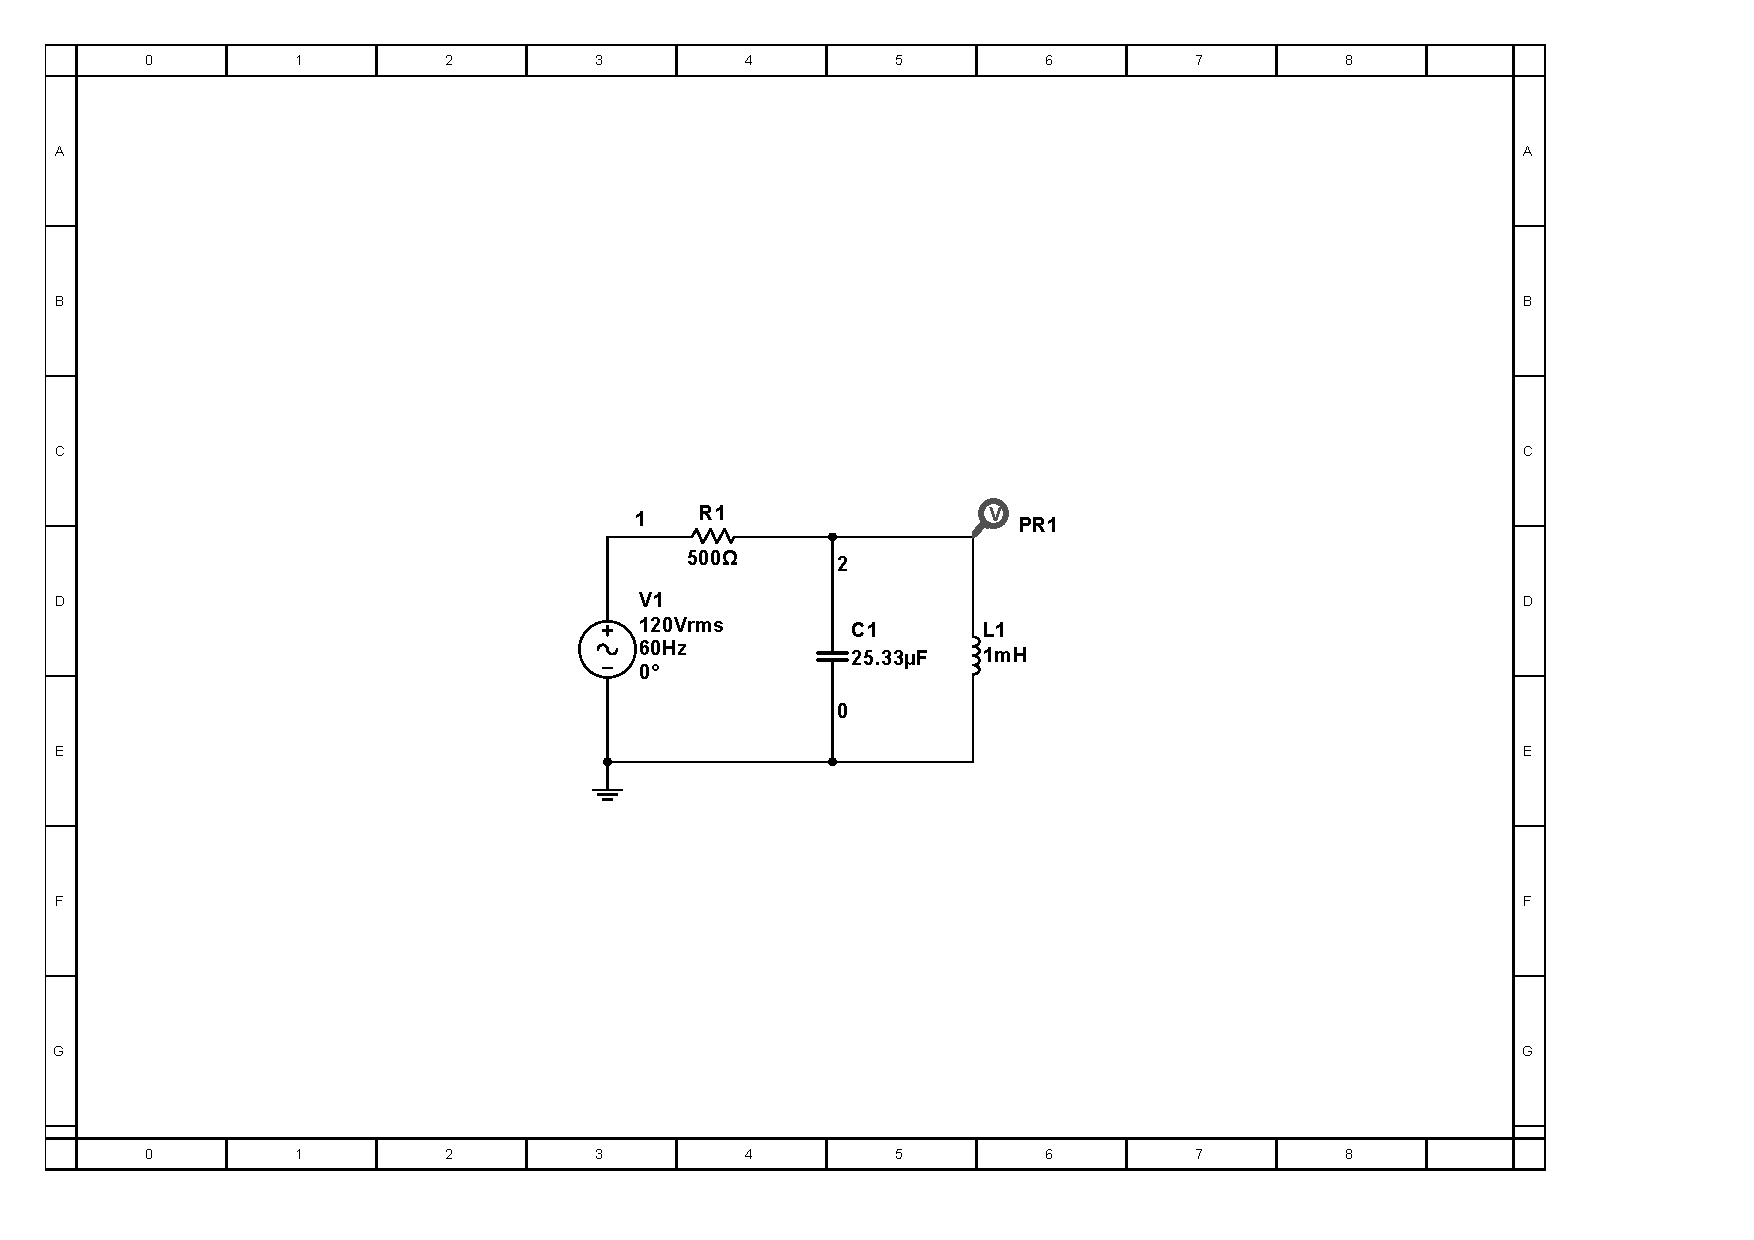
\includepdf[pages={1},angle=90]{电路设计/带通滤波器/带通滤波器电路图.pdf}

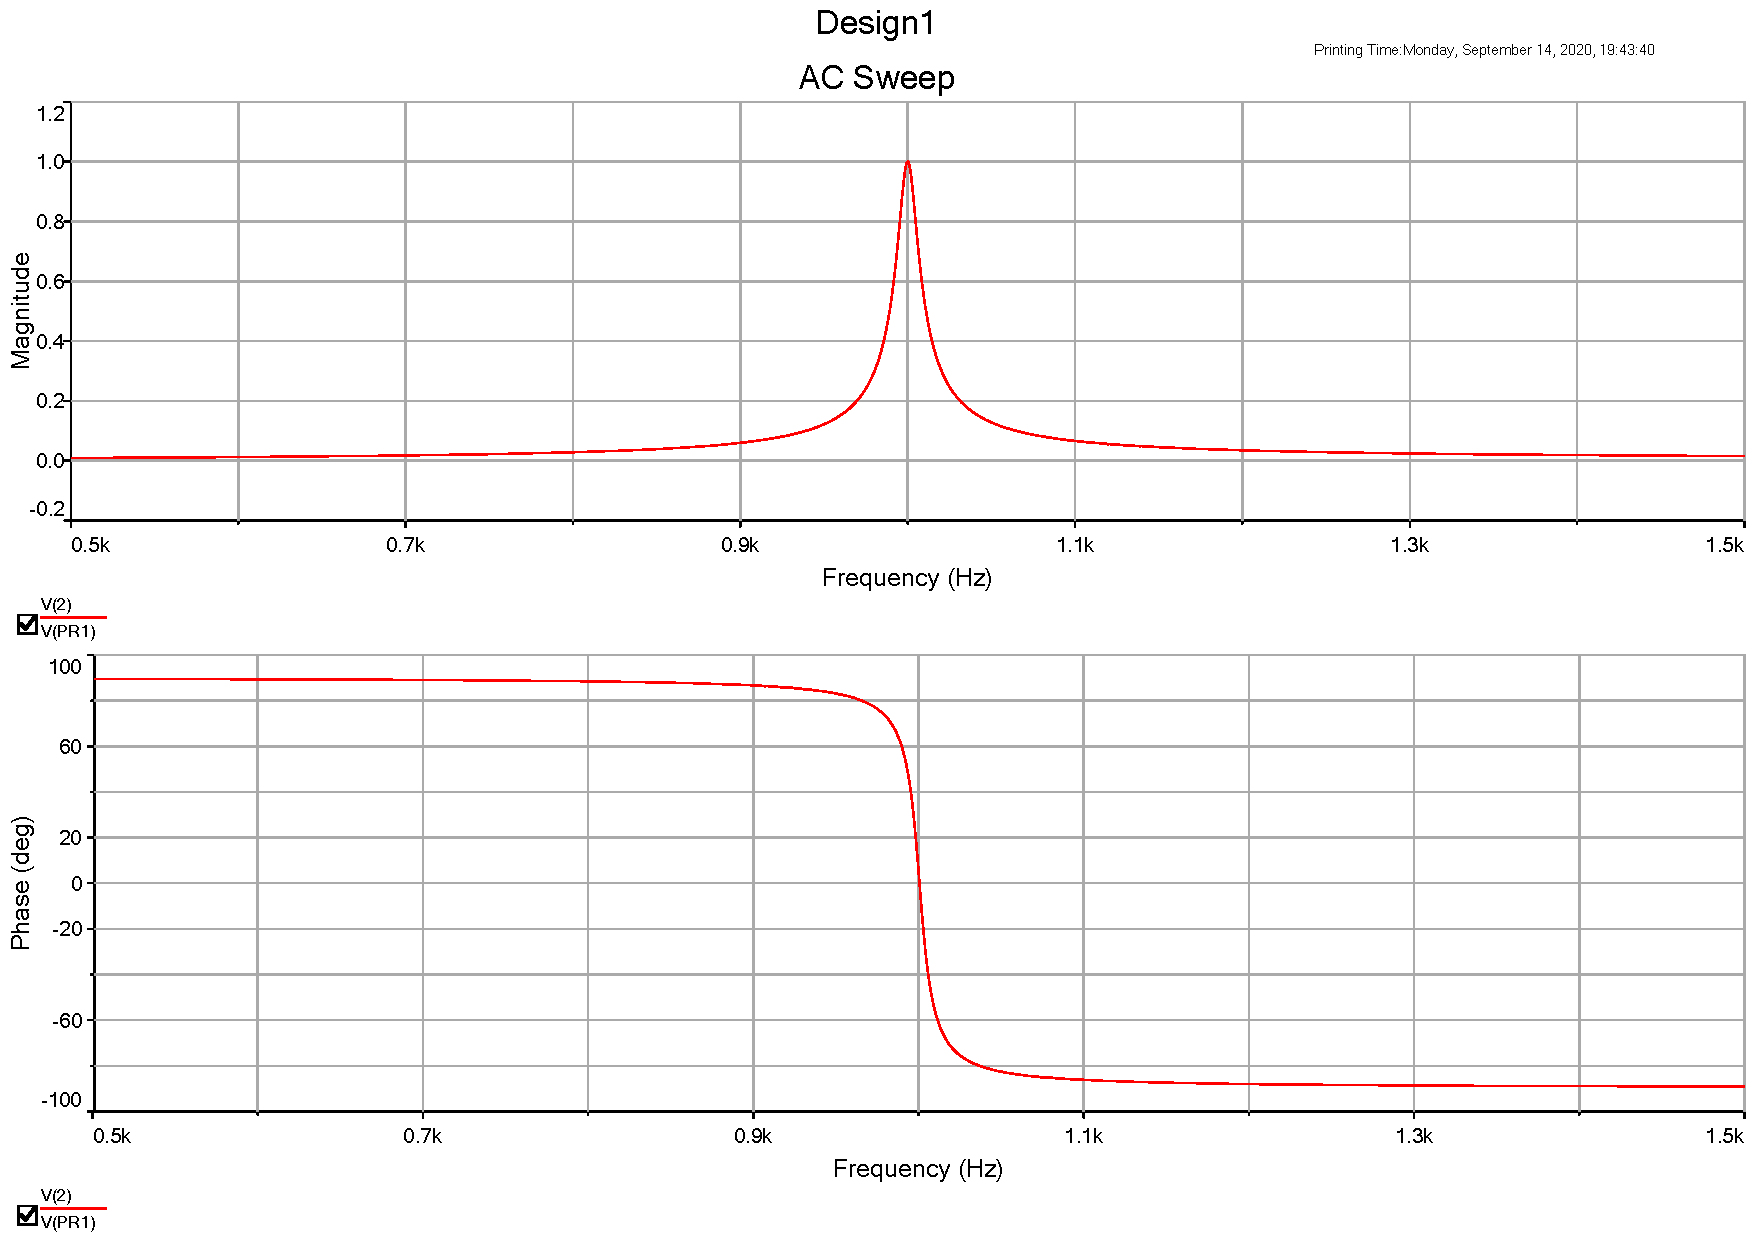
\includepdf[pages={1},angle=90]{电路设计/带通滤波器/带通滤波器频率相应.pdf}

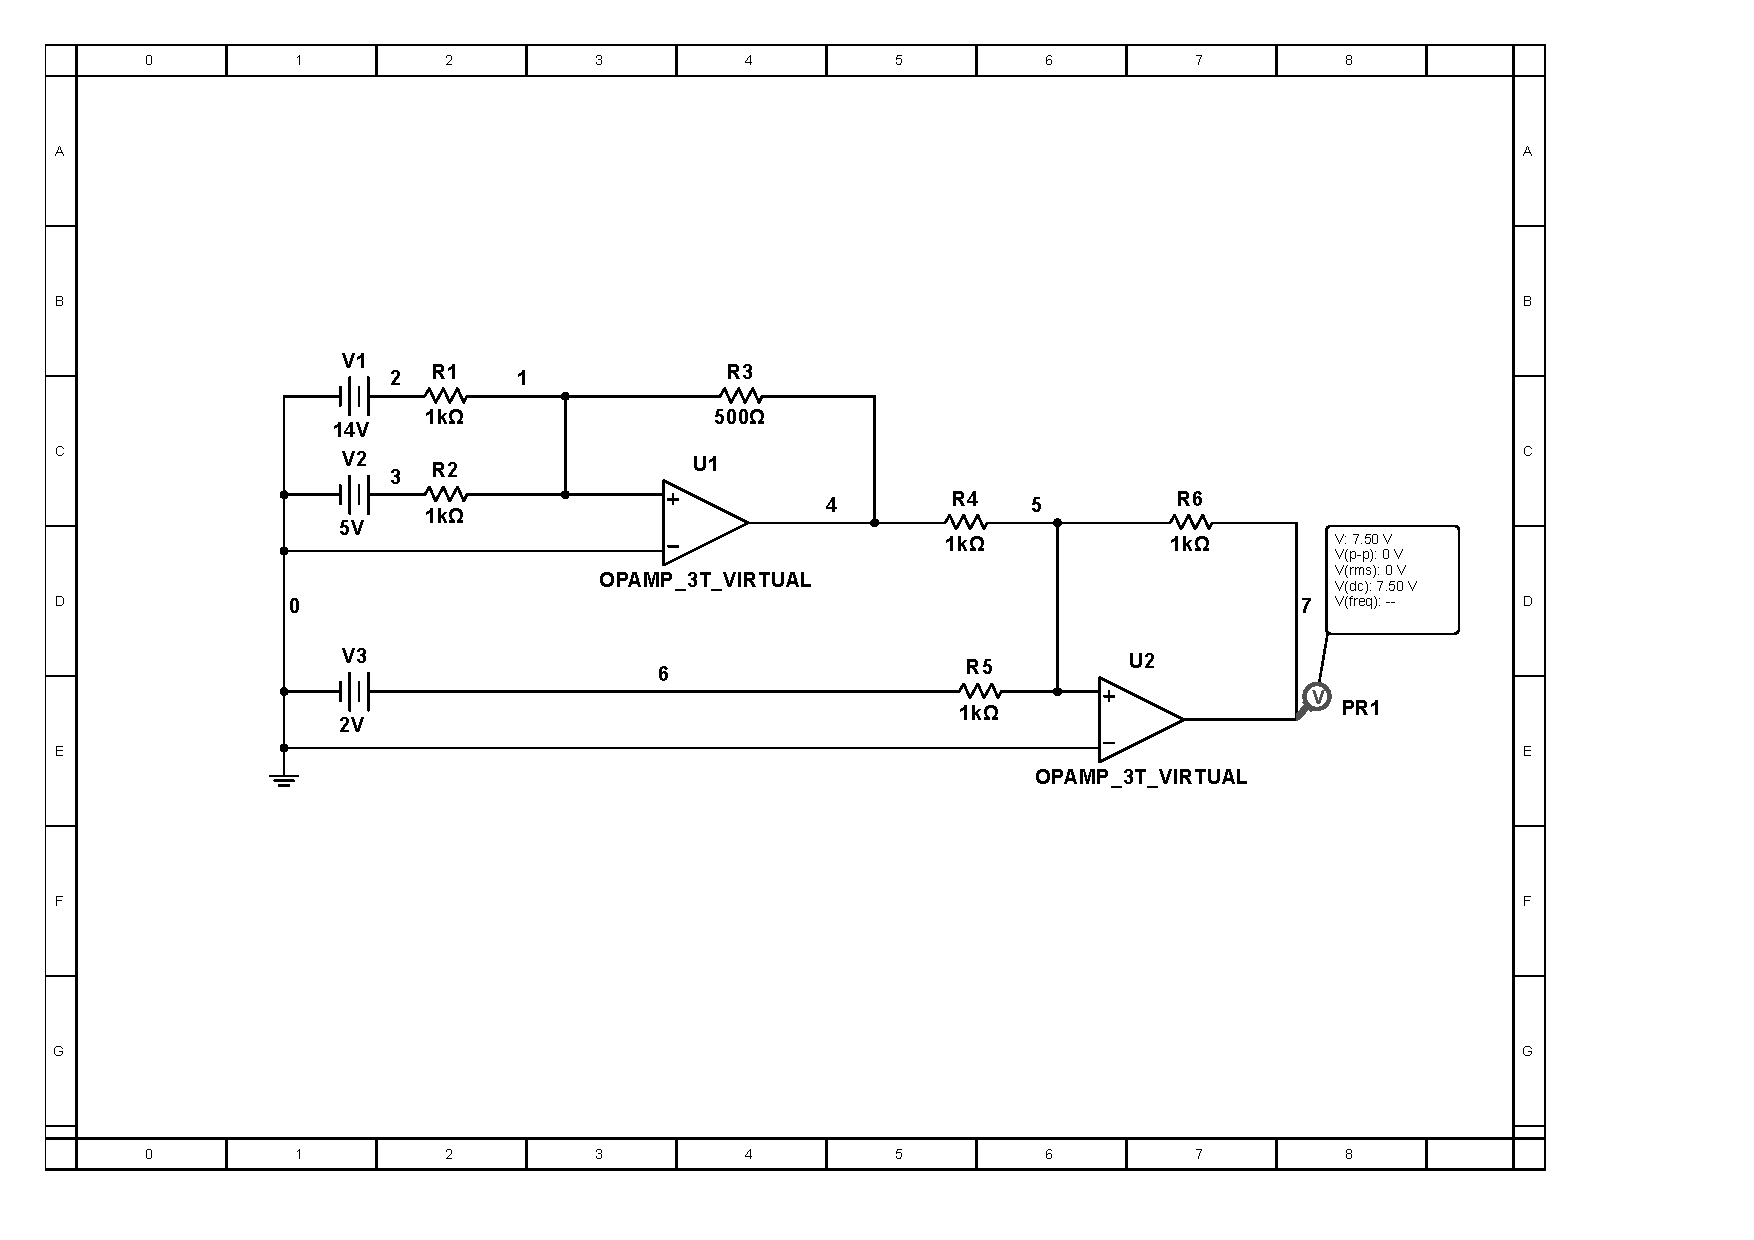
\includepdf[pages={1},angle=90]{电路设计/加减法电路/加减法电路电路图.pdf}

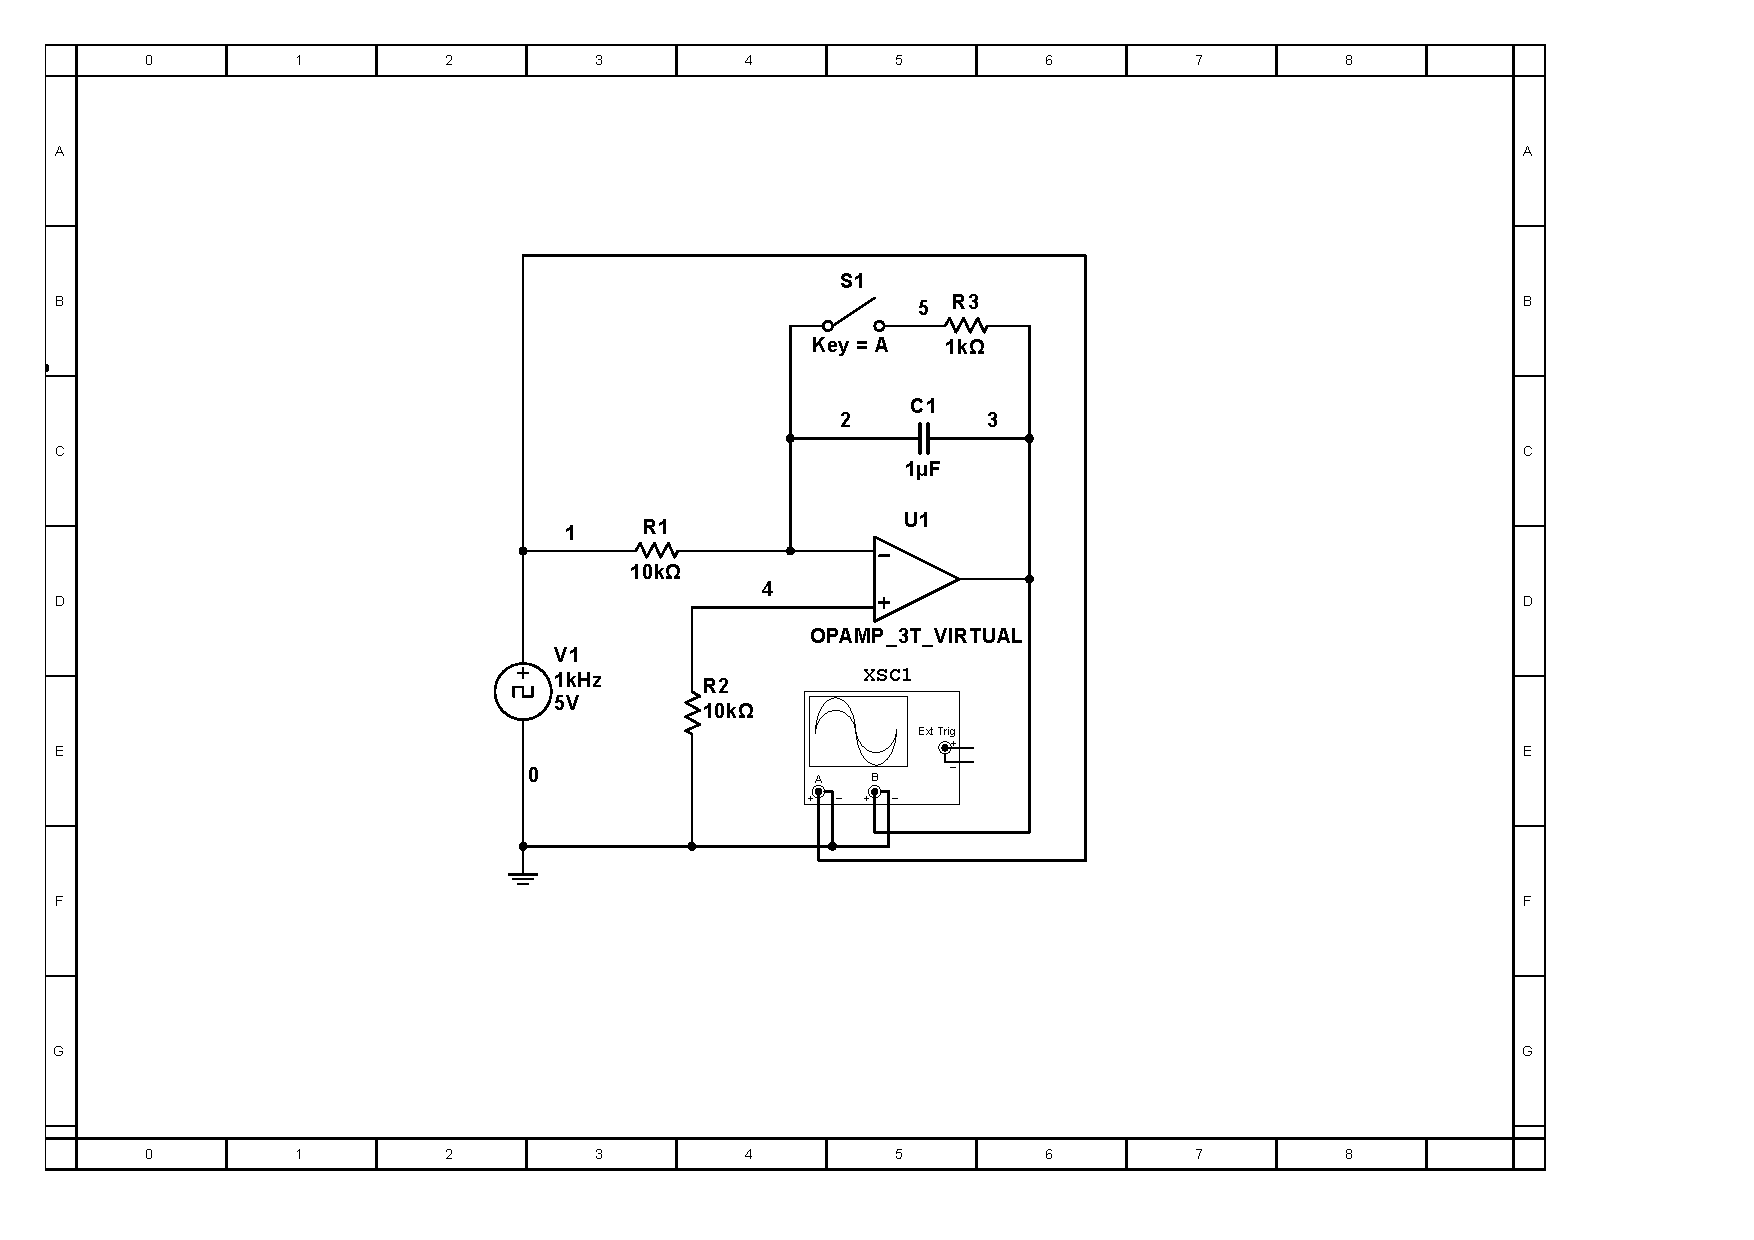
\includepdf[pages={1},angle=90]{电路设计/积分电路/积分电路电路图.pdf}

\begin{figure}[H]
  \centering
  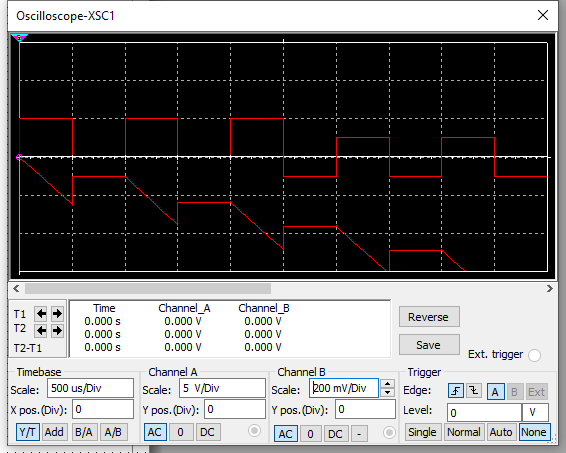
\includegraphics[width=0.75\linewidth]{电路设计/积分电路/积分电路无Rf.png}
  \caption{积分电路无Rf}
\end{figure}

\begin{figure}[H]
  \centering
  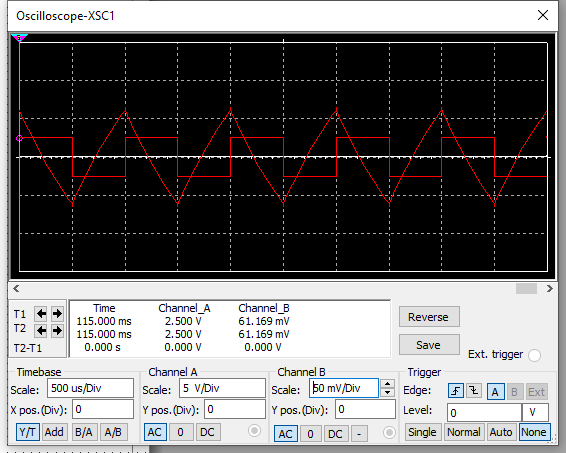
\includegraphics[width=0.75\linewidth]{电路设计/积分电路/积分电路有Rf.png}
  \caption{积分电路有Rf}
\end{figure}

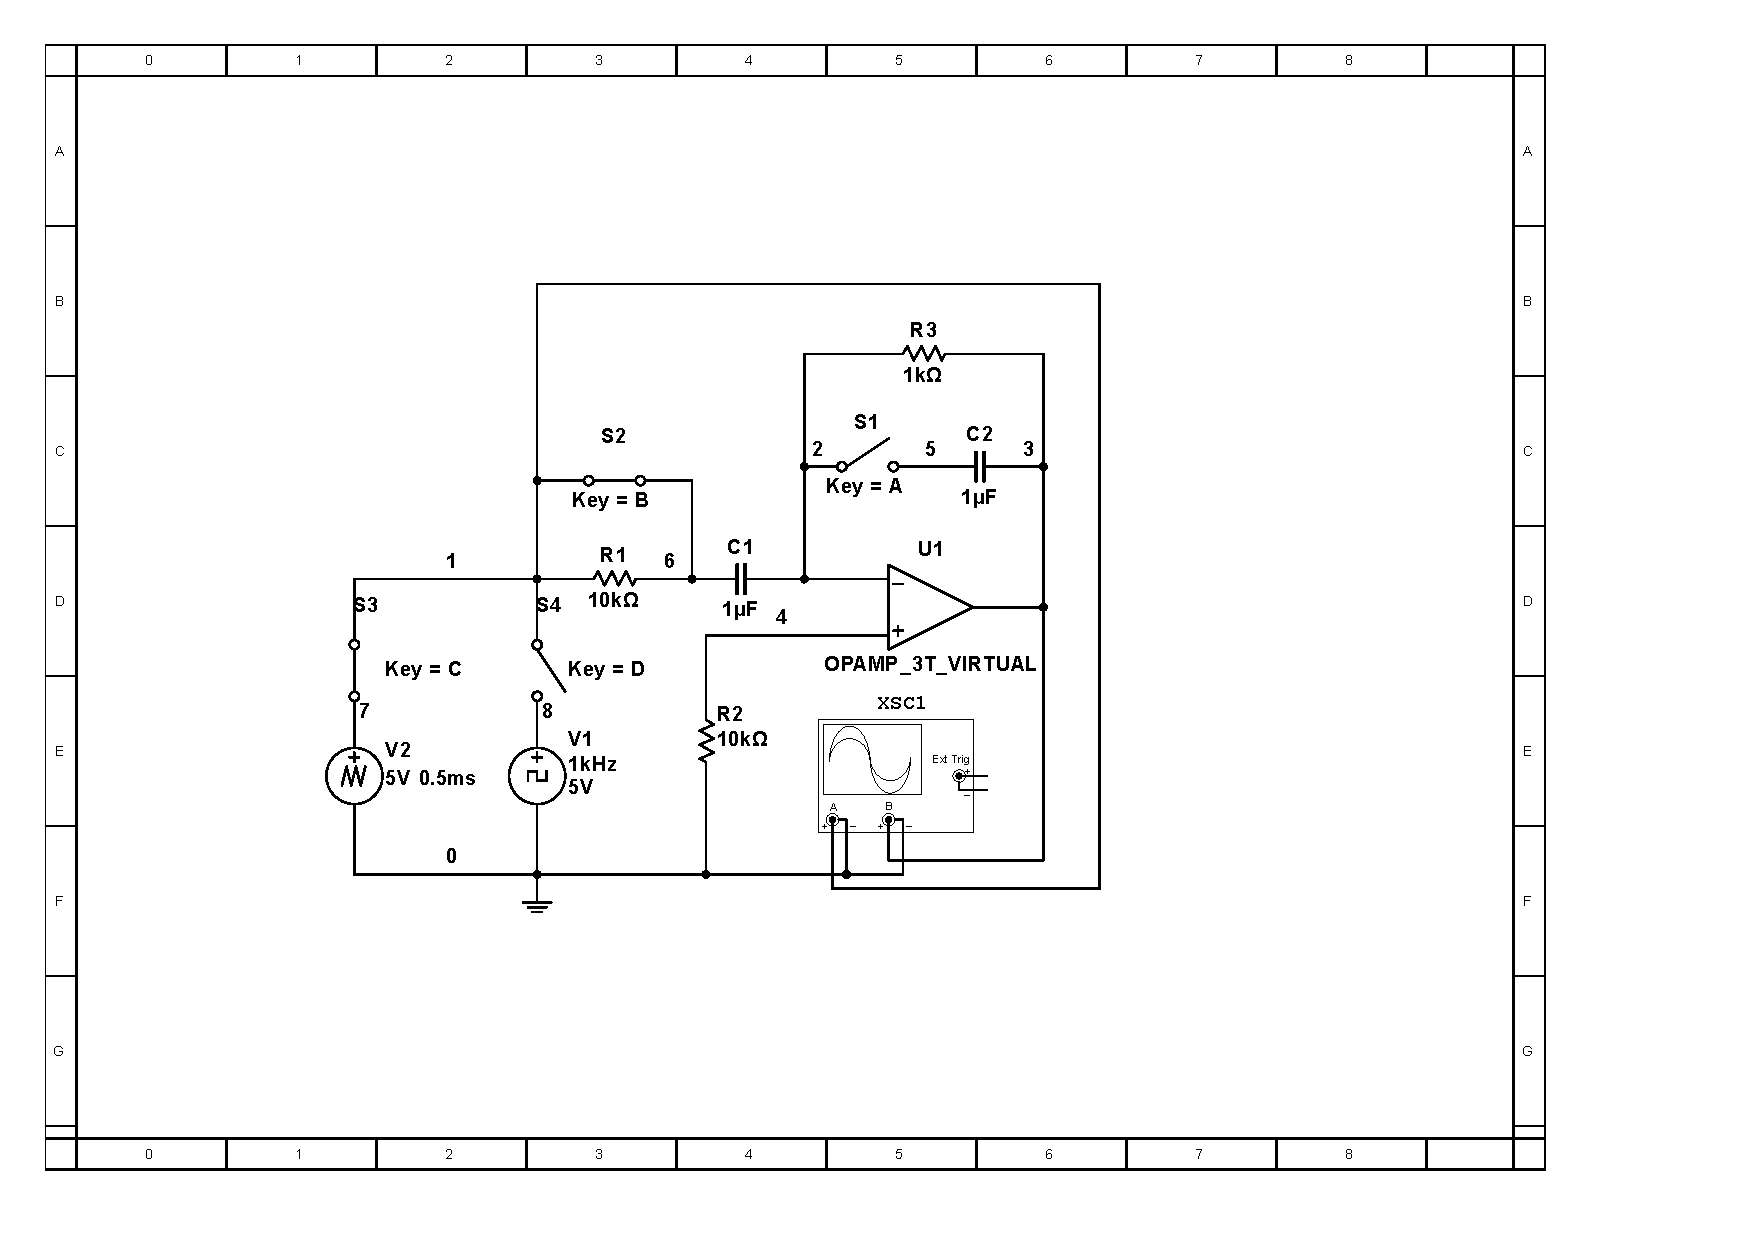
\includepdf[pages={1},angle=90]{电路设计/微分电路/微分电路电路图.pdf}

\begin{figure}[H]
  \centering
  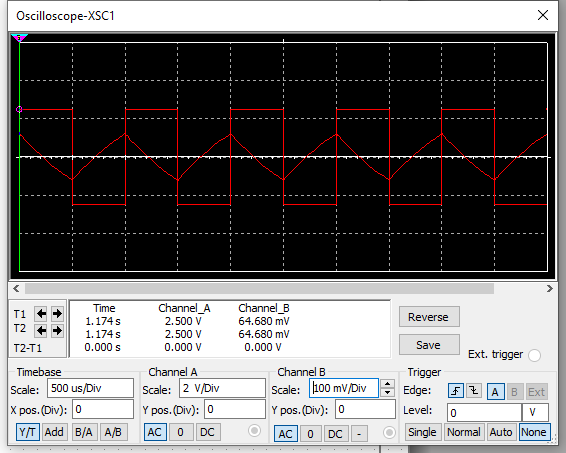
\includegraphics[width=0.75\linewidth]{电路设计/微分电路/微分电路方波有电阻有电容.png}
  \caption{微分电路方波有电阻有电容}
\end{figure}

\begin{figure}[H]
  \centering
  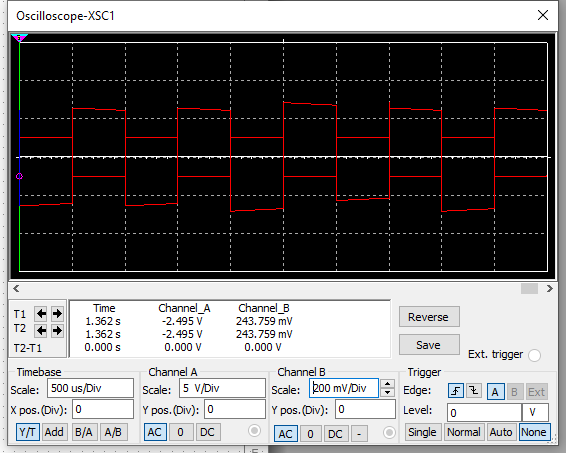
\includegraphics[width=0.75\linewidth]{电路设计/微分电路/微分电路方波有电阻无电容.png}
  \caption{微分电路方波有电阻无电容}
\end{figure}

\begin{figure}[H]
  \centering
  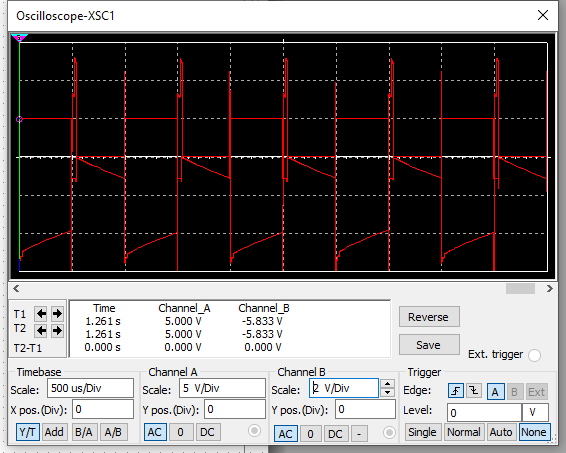
\includegraphics[width=0.75\linewidth]{电路设计/微分电路/微分电路方波无电阻有电容.png}
  \caption{微分电路方波无电阻有电容}
\end{figure}

\begin{figure}[H]
  \centering
  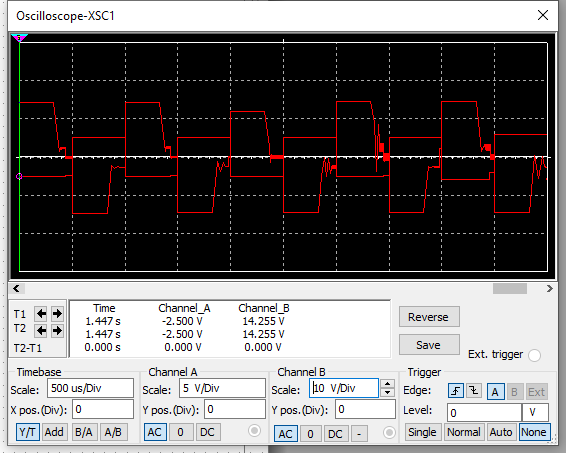
\includegraphics[width=0.75\linewidth]{电路设计/微分电路/微分电路方波无电阻无电容.png}
  \caption{微分电路方波无电阻无电容}
\end{figure}

\begin{figure}[H]
  \centering
  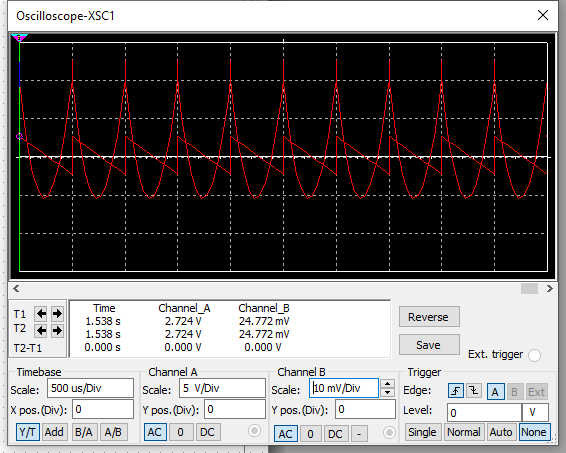
\includegraphics[width=0.75\linewidth]{电路设计/微分电路/微分电路三角波有电阻有电容.png}
  \caption{微分电路三角波有电阻有电容}
\end{figure}

\begin{figure}[H]
  \centering
  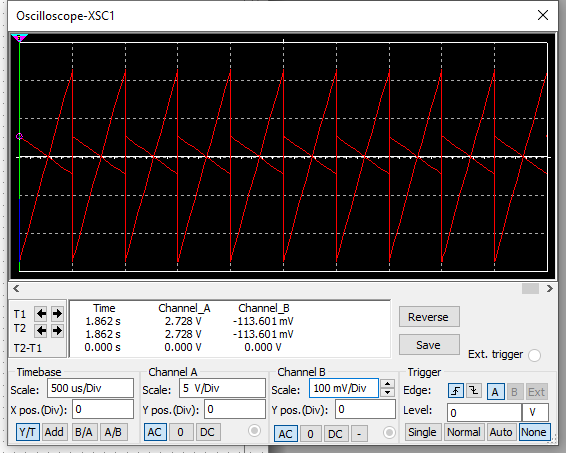
\includegraphics[width=0.75\linewidth]{电路设计/微分电路/微分电路三角波有电阻无电容.png}
  \caption{微分电路三角波有电阻无电容}
\end{figure}

\begin{figure}[H]
  \centering
  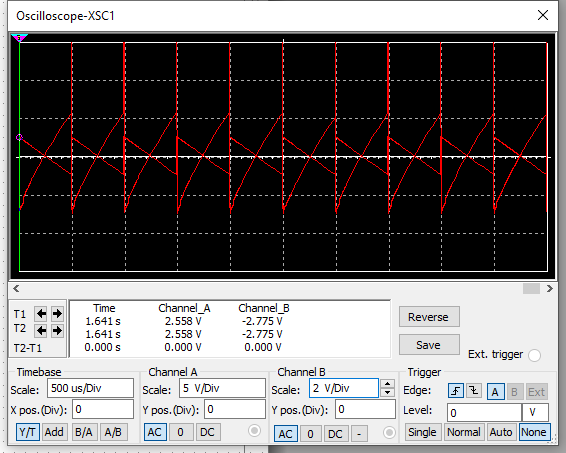
\includegraphics[width=0.75\linewidth]{电路设计/微分电路/微分电路三角波无电阻有电容.png}
  \caption{微分电路三角波无电阻有电容}
\end{figure}

\begin{figure}[H]
  \centering
  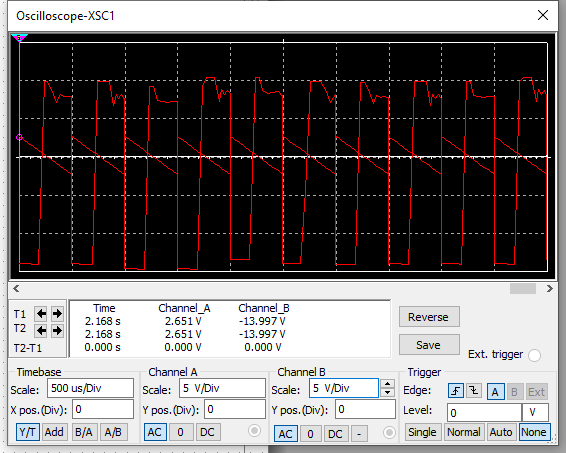
\includegraphics[width=0.75\linewidth]{电路设计/微分电路/微分电路三角波无电阻无电容.png}
  \caption{微分电路三角波无电阻无电容}
\end{figure}

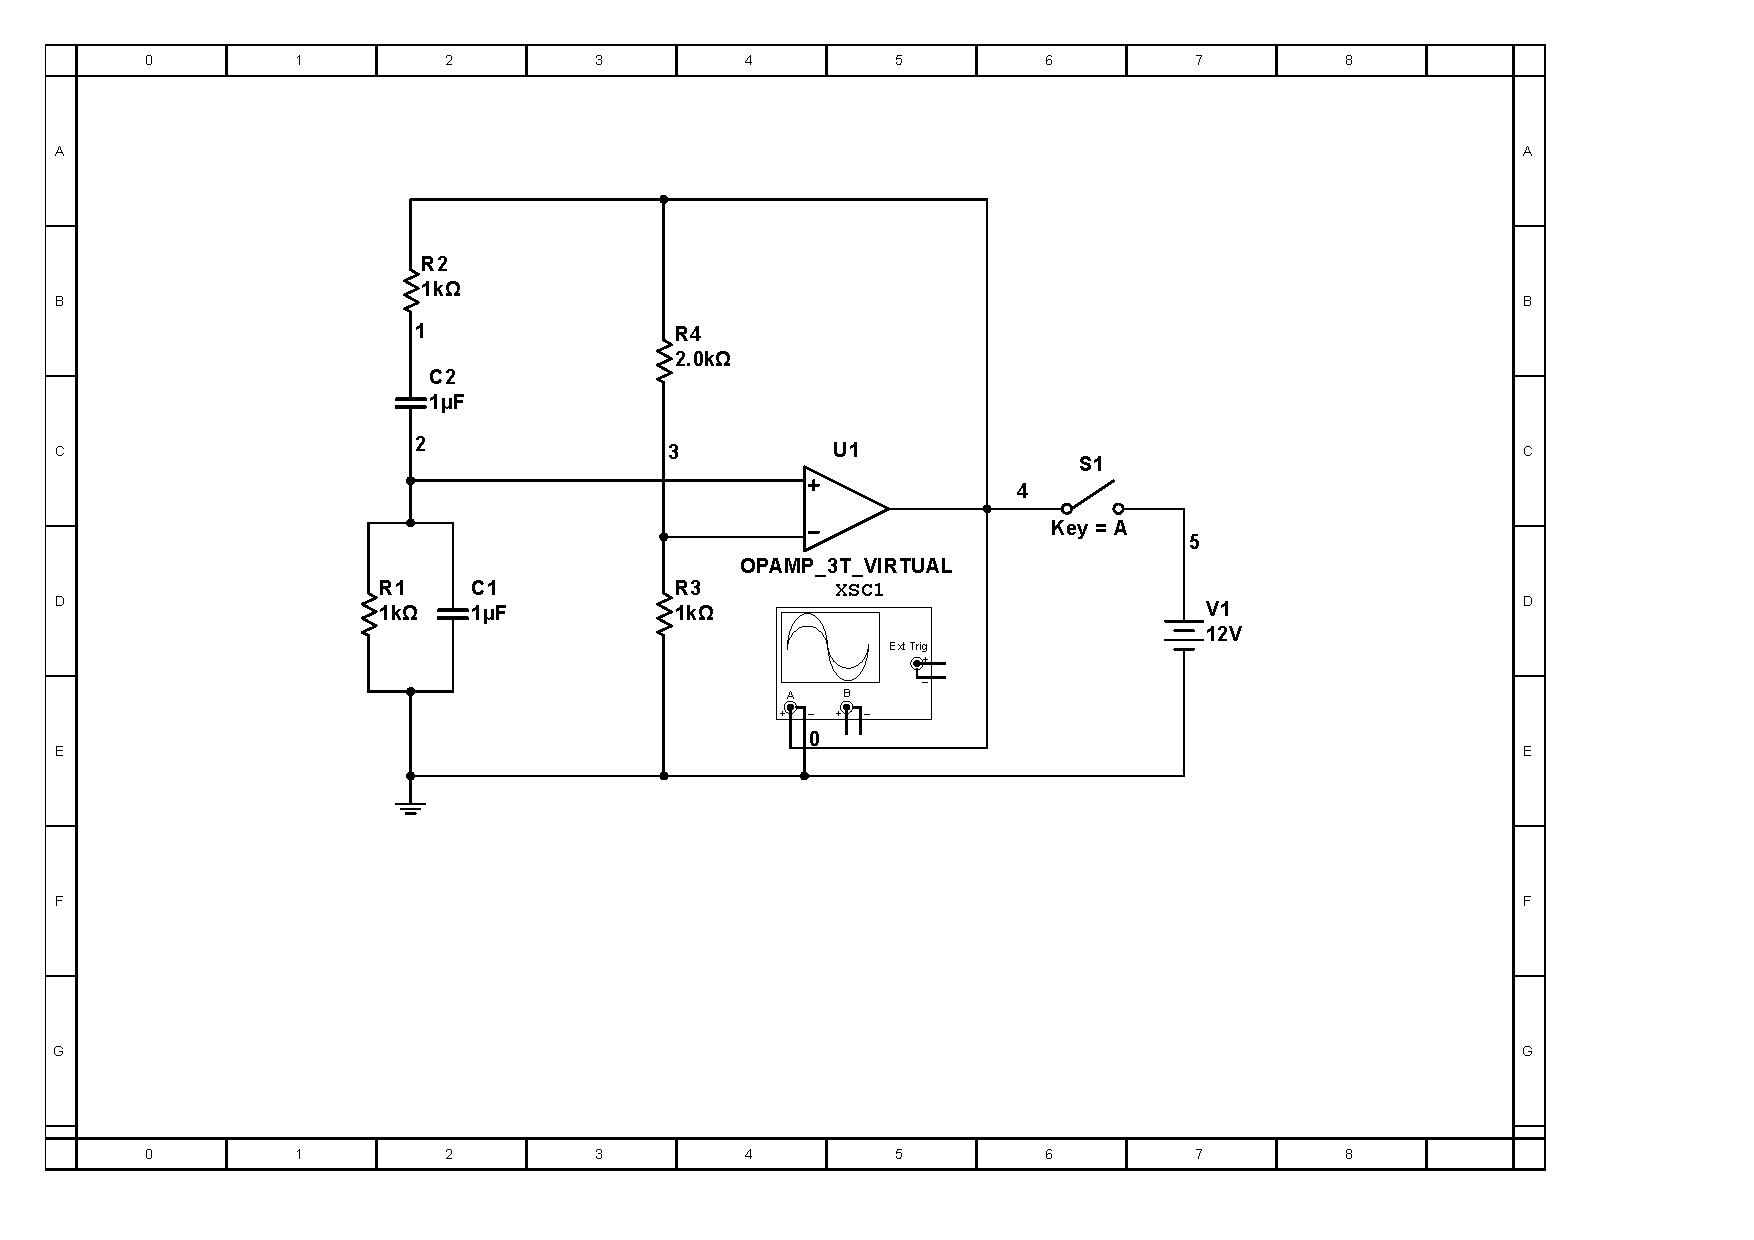
\includepdf[pages={1},angle=90]{电路设计/正弦波发生器/正弦波发生器电路图.pdf}

\begin{figure}[H]
  \centering
  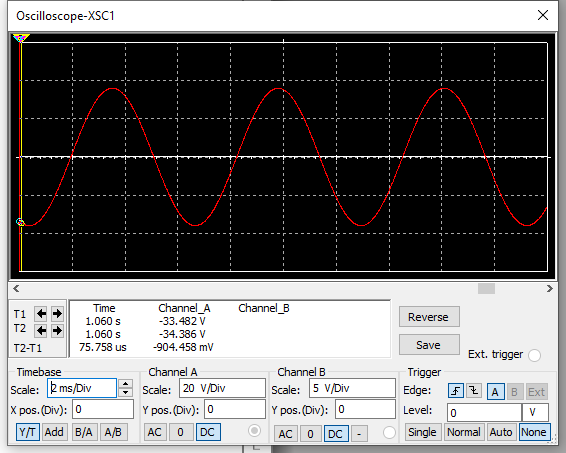
\includegraphics[width=0.75\linewidth]{电路设计/正弦波发生器/正弦波发生器示波器.png}
  \caption{正弦波发生器}
\end{figure}

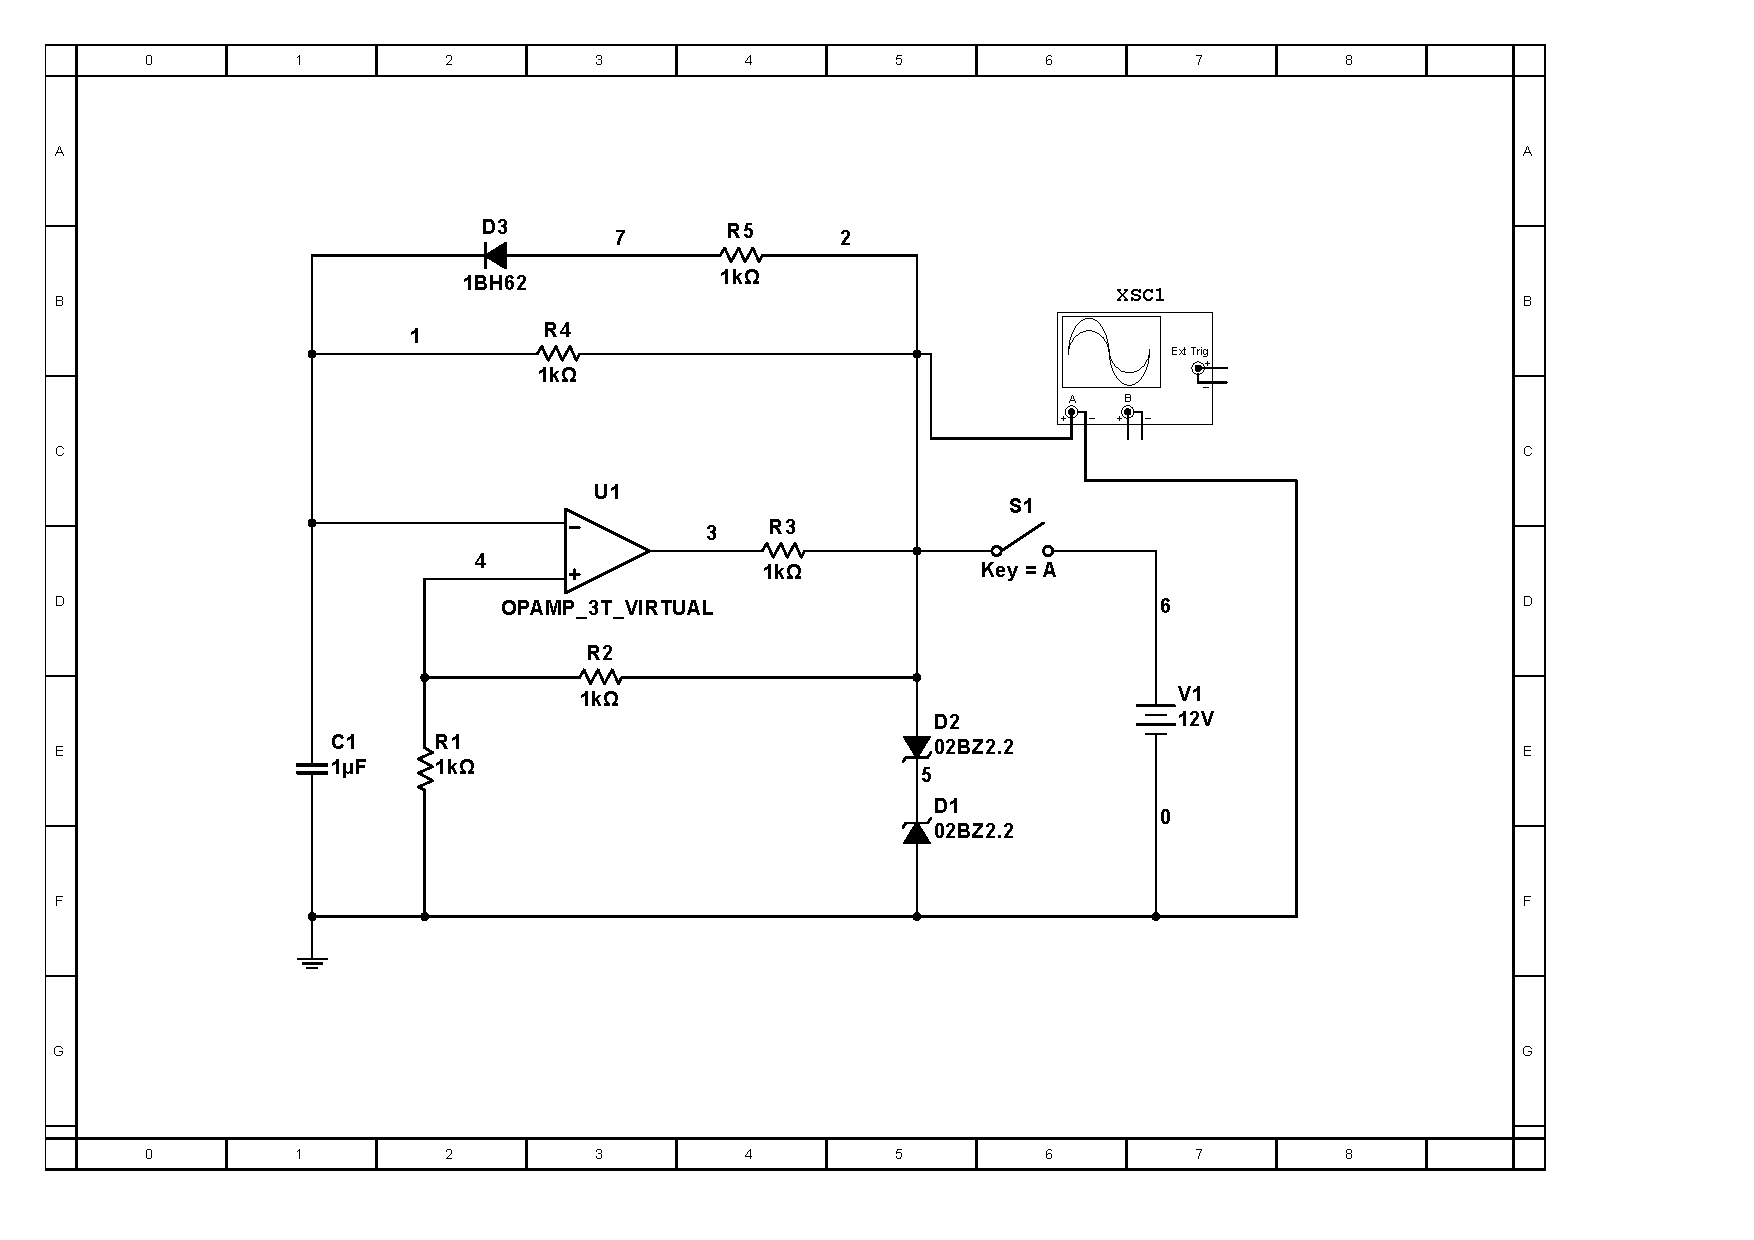
\includepdf[pages={1},angle=90]{电路设计/矩形波电路/矩形波电路电路图.pdf}

\begin{figure}[H]
  \centering
  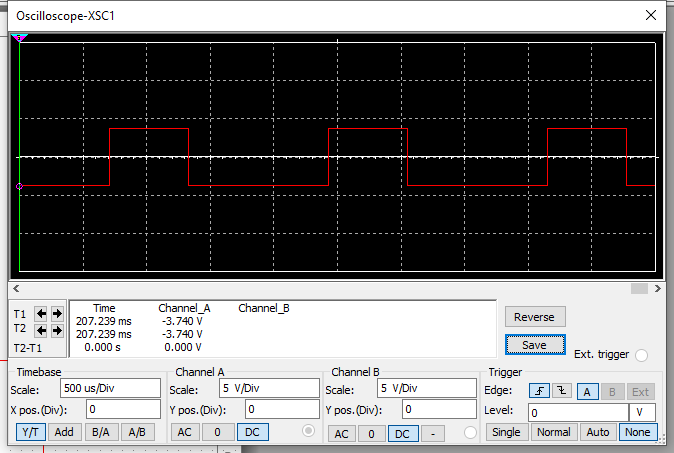
\includegraphics[width=0.75\linewidth]{电路设计/矩形波电路/矩形波电路示波器图像.png}
  \caption{矩形波电路}
\end{figure}

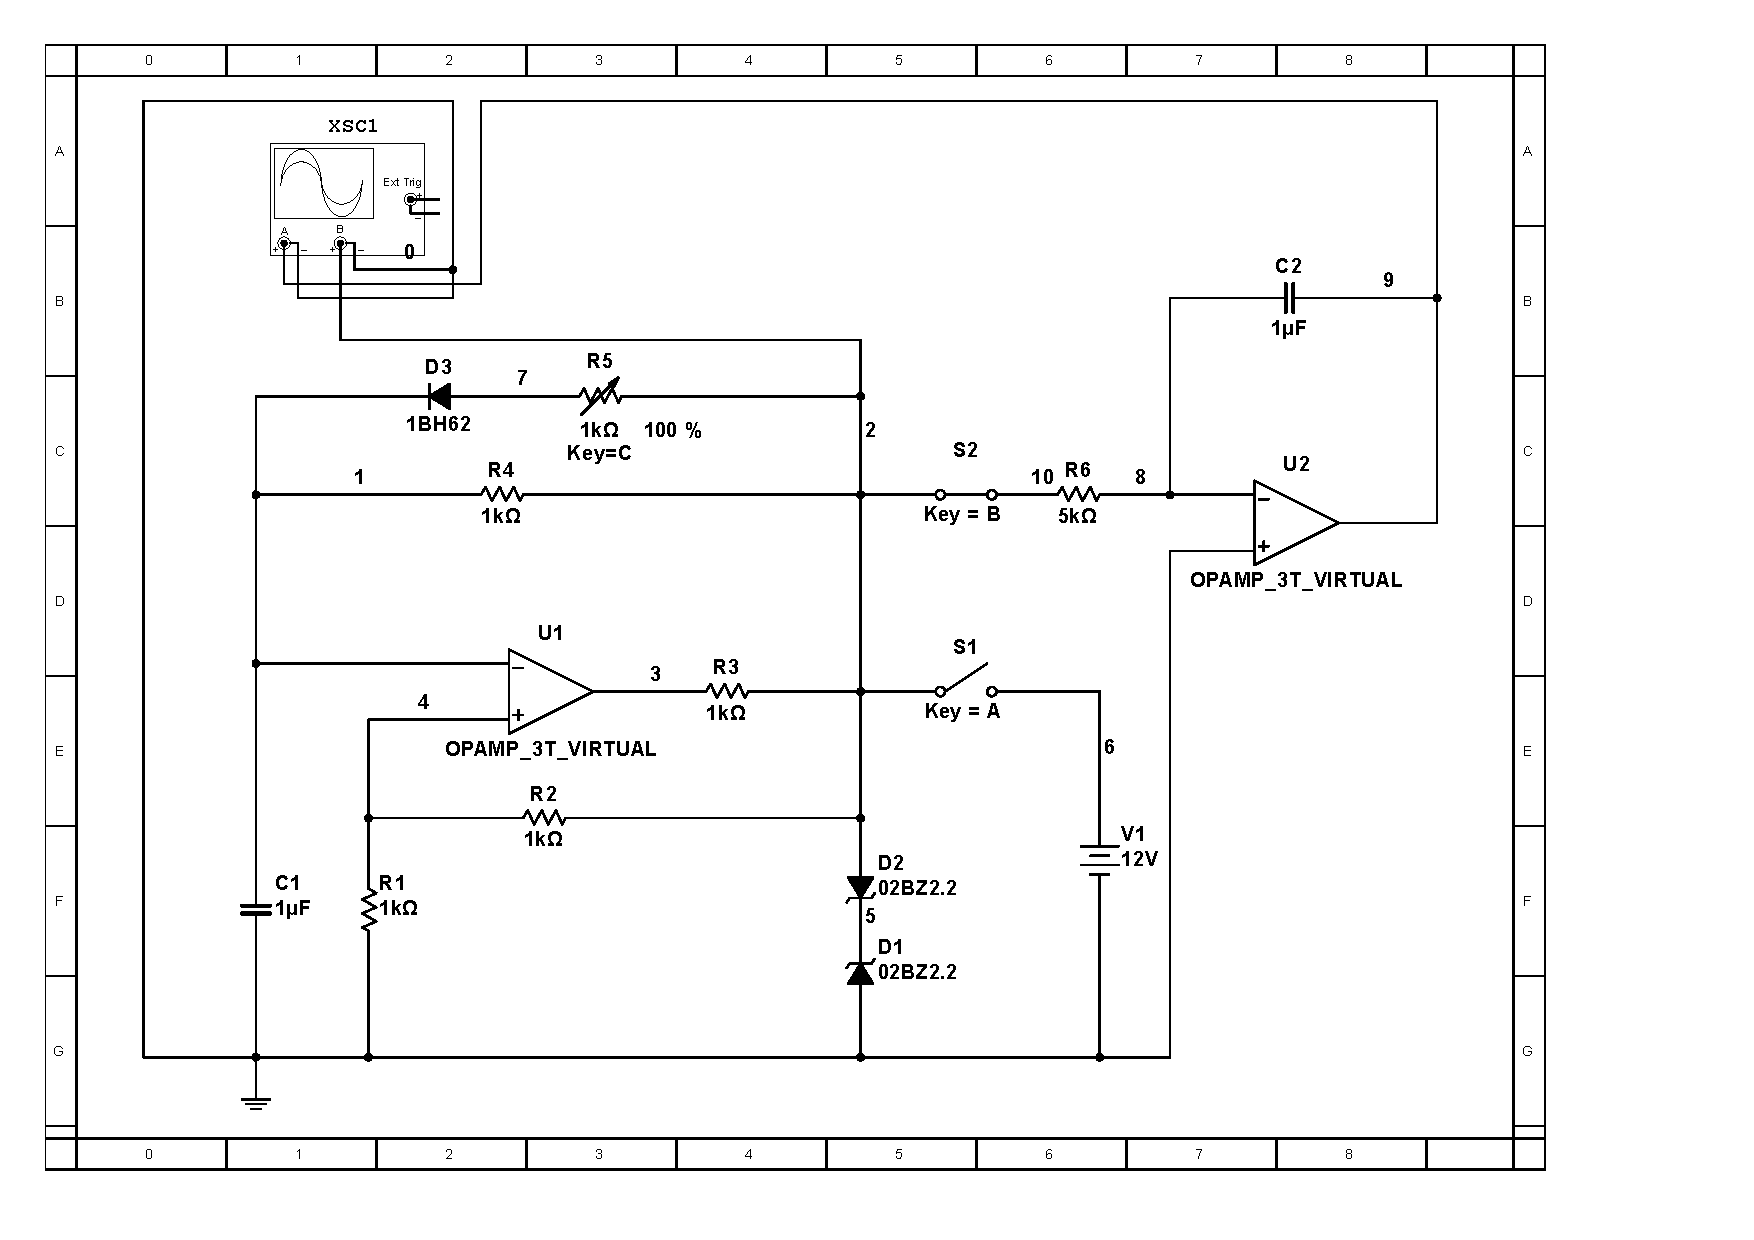
\includepdf[pages={1},angle=90]{电路设计/矩形-三角波发生电路/矩形-三角波发生电路电路图.pdf}

\begin{figure}[H]
  \centering
  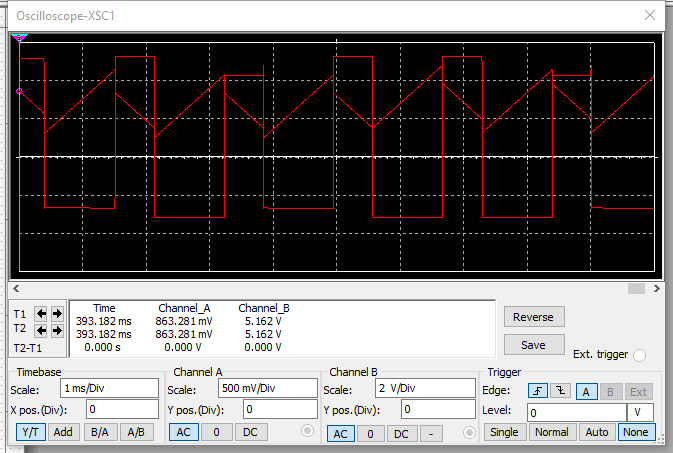
\includegraphics[width=0.75\linewidth]{电路设计/矩形-三角波发生电路/矩形-三角波发生电路示波器.png}
  \caption{矩形-三角波发生电路}
\end{figure}

\newpage

\section{实验内容与数据处理}

\subsection{实验结果的分析和结论}

第一个带通滤波器的实验,我们现场重新设计电路,电路图还是原来的电路图,但是电阻换成了$51 \Omega$,电感换成了$4.7 \mu H$,电容换成了$0.68 \mu F$,调整输入信号的频率,用示波器测量输出电压,最终绘制图像,得到如下结果

\begin{figure}[H]
  \centering
  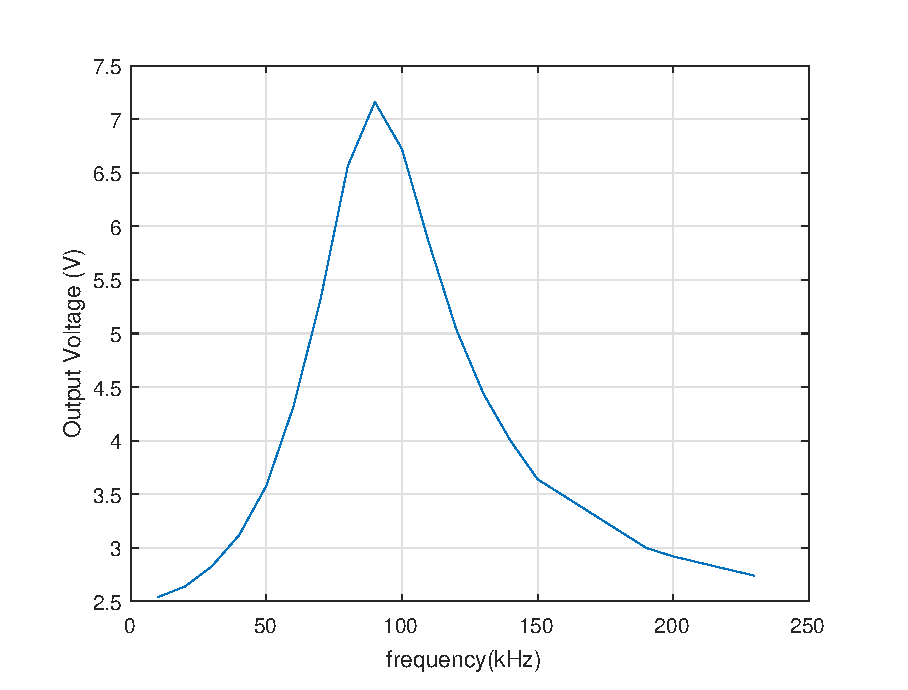
\includegraphics[width=0.9\linewidth]{figures/带通滤波器}
  \caption{带通滤波器输出电压随频率变化图像}
\end{figure}

理论上图像的峰值应当为89026Hz,实际和理论大致相同。

之后是运算放大器失调电压和电流的测量,测量的时候按照教材上的电路图搭建电路,当两个开关都闭合的时候,测得$U_{O1}=14.5 \si{mV}$,两个开关都断开时,测得$U_{O2}=9.5 \si{mV}$,因此输入失调电压为

\begin{equation*}
  \begin{aligned}
    U_{IO} &= \dfrac{R_1}{R_1 + R_f} U_{O1} = \dfrac{100 \si{\Omega}}{100 \si{\Omega} + 10 \si{k \Omega}} U_{O1} = 143 \si{\mu V}
  \end{aligned}
\end{equation*}

输入失调电流为

\begin{equation*}
  \begin{aligned}
    I_{IO} &= \left| U_{O2} - U_{O1} \right| \dfrac{R_1}{R_1 + R_f} \dfrac{1}{R_2} = \dfrac{100 \si{\Omega}}{100 \si{\Omega} + 10 \si{k \Omega}} \cdot \dfrac{1}{20 \si{k \Omega}} \left| U_{O2} - U_{O1} \right| = 2.47 \si{pA}    
  \end{aligned}
\end{equation*}

在测量开环放大倍数时,连接电路后测得$U_O = 16.2 \si{V}$,$U_I = 1.3 \si{V}$,因此开环差模电压增益为

\begin{equation*}
  \begin{aligned}
    A_{vd} = \left( 1 + \dfrac{R_1}{R_2}  \right) \left| \dfrac{U_O}{U_I}  \right| = \left( 1 + \dfrac{100 \si{k \Omega}}{100 \Omega}  \right) \left| \dfrac{U_O}{U_I}  \right| = 12474
  \end{aligned}
\end{equation*}

连接测量共模抑制比的电路,通电后测得$U_{oc}=2.12 \si{V}$,$U_{ic} = 2.12 \si{V}$,因此共模抑制比为

\begin{equation*}
  \begin{aligned}
    K_{CMR} = \dfrac{R_f}{R_1} \dfrac{U_{ic}}{U_{oc}} = \dfrac{100 \si{k \Omega}}{1 \si{k \Omega}} \dfrac{U_{ic}}{U_{oc}} = 100    
  \end{aligned}
\end{equation*}

加减法电路我们并没有做出来,但是我们使用万用表检查了下电路,发现这是因为运算放大器不是理想的。理论上运算放大器在闭环工作状态下,同相输入端和反向输入端的电压应当相等,但是我们用万用表测量后发现不相等。

微分电路我们完全按照之前设计的图纸搭建,整个搭建过程中没有出现什么大问题,下面是实验中得到的输入方波的图像

\begin{figure}[H]
  \centering
  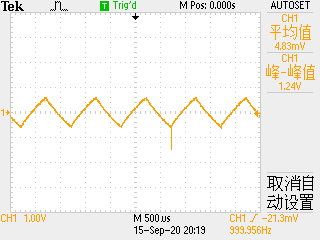
\includegraphics[width=0.96\linewidth]{电路图像/微分电路/输入方波/方波有电阻有电容}
  \caption{微分电路,方波,电阻电容都没有断开}
\end{figure}

\begin{figure}[H]
  \centering
  \begin{subfigure}{.32\textwidth}
    \centering
    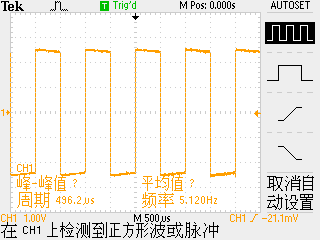
\includegraphics[width=\linewidth]{电路图像/微分电路/输入方波/方波有电阻无电容}
    \caption{微分电路,方波,断开电容}
  \end{subfigure}
  \begin{subfigure}{.32\textwidth}
    \centering
    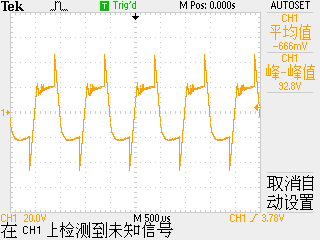
\includegraphics[width=\linewidth]{电路图像/微分电路/输入方波/方波无电阻有电容}
    \caption{微分电路,方波,断开电阻}
  \end{subfigure}
  \begin{subfigure}{.32\textwidth}
    \centering
    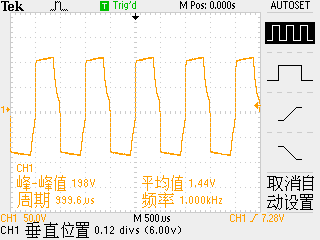
\includegraphics[width=\linewidth]{电路图像/微分电路/输入方波/方波无电阻无电容}
    \caption{微分电路,方波,断开电容电阻}
  \end{subfigure}
\end{figure}

输入锯齿波得到的图像如下

\begin{figure}[H]
  \centering
  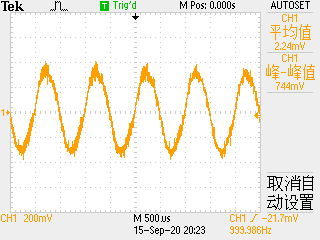
\includegraphics[width=0.96\linewidth]{电路图像/微分电路/输入锯齿波/三角波有电阻有电容}
  \caption{微分电路,锯齿波,电阻电容都没有断开}
\end{figure}

\begin{figure}[H]
  \centering
  \begin{subfigure}{.32\textwidth}
    \centering
    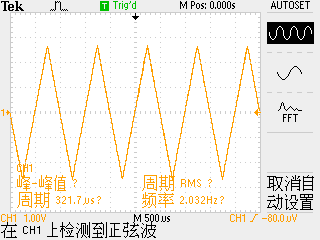
\includegraphics[width=\linewidth]{电路图像/微分电路/输入锯齿波/三角波有电阻无电容}
    \caption{微分电路,锯齿波,断开电容}
  \end{subfigure}
  \begin{subfigure}{.32\textwidth}
    \centering
    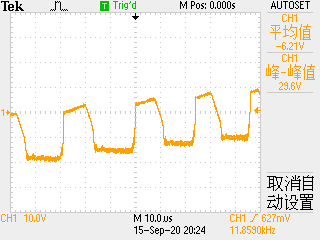
\includegraphics[width=\linewidth]{电路图像/微分电路/输入锯齿波/三角波无电阻有电容}
    \caption{微分电路,锯齿波,断开电阻}
  \end{subfigure}
  \begin{subfigure}{.32\textwidth}
    \centering
    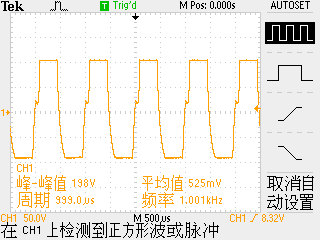
\includegraphics[width=\linewidth]{电路图像/微分电路/输入锯齿波/三角波无电阻无电容}
    \caption{微分电路,锯齿波,断开电容电阻}
  \end{subfigure}
\end{figure}

之后是积分电路,按照之前设计的搭建好后,有反馈电阻时得到了下面的图像,没有反馈电阻电路根本没有图像,示波器只有一条直线。这是因为没有那个电阻电容没有办法正常放电,电容上的电压只会越来越大,直至运算放大器达到饱和电压,从此以后只输出饱和电压。最开始通电的时候应当能看见图像是锯齿波但是在不停地向下移动,但是交流电频率太高无法捕捉到开始的几个周期,因为一个周期的时间太短了。

\begin{figure}[H]
  \centering
  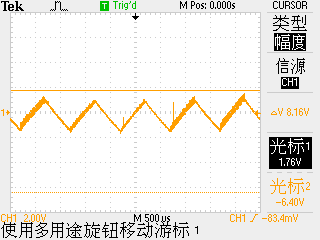
\includegraphics[width=0.75\linewidth]{电路图像/积分电路/积分电路有反馈电阻}
  \caption{积分电路,有反馈电阻,输入方波信号}
\end{figure}

最后是我设计的RC正弦波振荡电路,设计好之后先在输出端通直流电,一段时间后拿掉直流电源,使用示波器测量输出端,测到的图像如下

\begin{figure}[H]
  \centering
  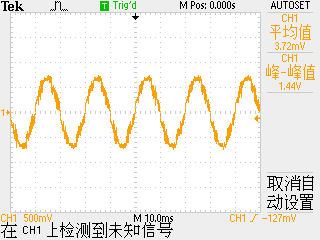
\includegraphics[width=0.75\linewidth]{电路图像/正弦波振荡电路/正弦波电路振荡图}
  \caption{正弦波振荡电路测出的示波器图像}
\end{figure}

\subsection{实验中遇到的问题及解决方法}

实验中问题最大的是第一个设计带通滤波器的实验,刚开始我们找了好久电路是不是有问题,然后换了元器件,问题没有解决,又换了几次解决了。可能是实验材料里有一些损坏的元器件。

\section{参考文献}
\begin{itemize}[leftmargin=0pt]
  \item[] 近代物理实验讲义
\end{itemize}
\end{document} 
